\documentclass[obeyspaces,spaces,hyphens]{beamer}
\usepackage[utf8]{inputenc}
\usepackage{minted}
\usepackage[english,russian]{babel}
\mode<presentation>
\usetheme{Bootlin}

\newcommand{\codehack}[1]{{\usebeamercolor[fg]{code} {\tt #1}}}

\title{Device Tree for Dummies}
\authors{Thomas Petazzoni}
\institute{Bootlin}

\usepackage{hyperref}

\begin{document}

\begin{frame}
  \begin{center}
    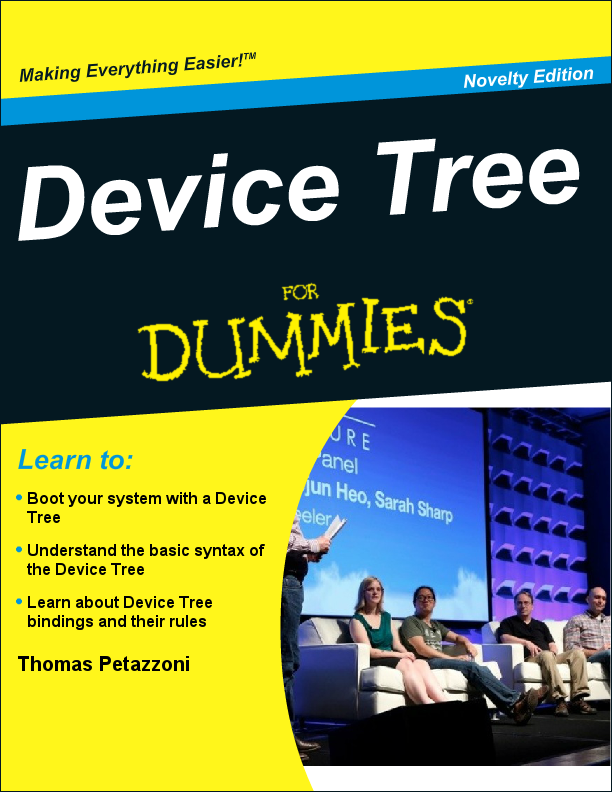
\includegraphics[height=0.95\textheight]{device-tree-for-dummies.png}
  \end{center}
\end{frame}

\begin{frame}{Thomas Petazzoni}
  \begin{itemize}
  \item Технический директор и инженер по встроенному Linux в Bootlin
    \begin{itemize}
    \item {\bf Разработка} встроенного ядра Linux и разработка драйверов, системная интеграция, оптимизация времени загрузки и энергопотребления, консультации и т. Д.
    \item {\bf Обучение} по встроенному Linux {\ bf}, обучение по разработке драйверов для Linux и обучение по разработке системы Android, материалы доступны под свободной лицензии Creative Commons.
    \item \url{http://bootlin.com}
    \end{itemize}
  \item Сотрудничество
    \begin{itemize}
    \item {\bf Поддержка ядра для Marvell Armada} ARM SoC от Marvell
    \item Основной участник {\ bf Buildroot}, простой и быстрой встроенной системы сборки Linux с открытым исходным кодом.
    \end{itemize}
  \item Живет в {\ bf Тулузе}, на юго-западе Франции.
  \end{itemize}
\end{frame}

\begin{frame}{Agenda}
  \begin{itemize}
  \item Напоминание о платформах ARM
   \item Пользовательская перспектива: загрузка с помощью дерева устройств
   \item Базовый синтаксис и компиляция дерева устройств
   \item Простой пример фрагмента дерева устройств
   \item Общая организация дерева устройств
   \item Примеры использования дерева устройств
   \item Общие сведения о дереве устройств в Linux
  \end{itemize}
\end{frame}

\begin{frame}{Напоминание о платформах ARM}
  \begin{itemize}
  \item {\bf ARM} (компания) разрабатывает ядра ЦП: набор команд, MMU, кеши и т. д.
    \begin{itemize}
    \item Они не продают оборудование
    \end{itemize}
  \item {\bf Поставщики кремния} покупают дизайн ядра ЦП у ARM, и  вокруг него добавьте несколько {\em периферийных устройств}, либо разработанных  внутри компании или купленные у третьих лиц
    \begin{itemize}
    \item Texas Instruments, Atmel, Marvell, Freescale, Qualcomm,
      Nvidia, etc.
    \item Они продают {\em Систеиы на кристалле} или {\em SoC}
    \end{itemize}
  \item {\bf Производители систем} проектируют настоящую плату с одним или несколькими процессорами и несколькими встроенными периферийными устройствами.
  \end{itemize}
\end{frame}

\begin{frame}{Схематическое изображение платформы ARM}
  \begin{center}
    \includegraphics[width=\textwidth]{arm-architecture.pdf}
  \end{center}
\end{frame}

\begin{frame}{Обнаруживаемое и не обнаруживаемое оборудование}
  \begin{itemize}
  \item Некоторые автобусы имеют функции динамического обнаружения.
    \begin{itemize}
    \item USB, PCI
    \item Позволяет перечислять устройства на шине, запрашивать их характеристики во время выполнения.
    \item Не нужно заранее знать, что в шине
    \end{itemize}
  \item Но многие шины не имеют таких возможностей.
    \begin{itemize}
    \item Устройства с отображением памяти внутри SoC, I2C, SPI, SDIO, etc.
    \item Система должна заранее знать, где находятся различные устройства, и их характеристики.
    \end{itemize}
  \end{itemize}
\end{frame}

\begin{frame}{Перспектива пользователя: до дерева устройств}
  \begin{itemize}
  \item Ядро содержит полное описание оборудования.
  \item Загрузчик загружает единственный двоичный файл, образ ядра, и выполняет его.
    \begin{itemize}
    \item \code{uImage} or \code{zImage}
    \end{itemize}
  \item Загрузчик подготавливает дополнительную информацию, которая называется
     \code {ATAGS}, адрес которого передается ядру через
     зарегистрироваться \code {r2}
    \begin{itemize}
    \item Содержит такую информацию, как размер и расположение памяти, командная строка ядра и т. Д.
    \end{itemize}
  \item Загрузчик сообщает ядру, на какой плате оно загружается, с помощью целого числа {\em machine type}, переданного в регистре
    \code{r1}.
  \item U-Boot command: \code{bootm <kernel img addr>}
  \item Переменная Barebox: \code{bootm.image}
  \end{itemize}
\end{frame}

\begin{frame}{Перспектива пользователя: до дерева устройств}
  \begin{center}
    \includegraphics[height=0.6\textheight]{booting-without-dt.pdf}
  \end{center}
\end{frame}

\begin{frame}{Перспектива пользователя: загрузка с помощью дерева устройств}
  \begin{itemize}
  \item Ядро больше не содержит описания оборудования, оно находится в отдельном двоичном файле: {\em blob дерева устройств}
  \item The bootloader loads two binaries: the kernel image and the
    {\em DTB}
    \begin{itemize}
    \item Образ ядра находится \code{uImage} или в \code{zImage}
    \item DTB находится в \code{arch/arm/boot/dts}, по одному на плату.
    \end{itemize}
  \item Загрузчик передает адрес DTB через \code {r2}. Предполагается настроить DTB с помощью информации о памяти, командной строки ядра и, возможно, другой информации.
  \item No more {\em machine type}.
  \item U-Boot command: \code{boot[mz] <kernel img addr> - <dtb addr>}
  \item Переменные Barebox: \code{bootm.image}, \code{bootm.oftree}
  \end{itemize}
\end{frame}

\begin{frame}{Перспектива пользователя: загрузка с помощью дерева устройств}
  \begin{center}
    \includegraphics[height=0.6\textheight]{booting-with-dt.pdf}
  \end{center}
\end{frame}

\begin{frame}[fragile]{С точки зрения пользователя: режим совместимости для загрузки DT
}
  \begin{itemize}
  \item Некоторые загрузчики не имеют специальной поддержки для дерева устройств, или версия, используемая на конкретном устройстве, слишком старая для такой поддержки.
  \item Для облегчения перехода был добавлен {\em механизм совместимости}: \code{CONFIG_ARM_APPENDED_DTB}.
    \begin{itemize}
    \item Он говорит ядру искать DTB сразу {\em после образа ядра}.
    \item Встроенного правила Makefile для создания такого ядра нет, поэтому нужно вручную сделать:
      \begin{block}{}
        \begin{minted}[fontsize=\scriptsize]{bash}
cat arch/arm/boot/zImage arch/arm/boot/dts/myboard.dtb > my-zImage
mkimage ... -d my-zImage my-uImage
\end{minted}
\end{block}
\end{itemize}
  \item Кроме того, дополнительная опция
    \code{CONFIG_ARM_ATAG_DTB_COMPAT} сообщает ядру, что необходимо прочитать информацию {\em ATAGS} из загрузчика и обновить DT, используя их.
  \end{itemize}
\end{frame}

\begin{frame}{Что такое дерево устройств?}
  \begin{itemize}
  \item Цитата из {\em Power.org Standard for Embedded Power
      Architecture Platform Requirements (ePAPR)}
    \begin{itemize}
    \item EPAPR определяет концепцию, называемую деревом устройств, для описания оборудования системы. Программа загрузки загружает дерево устройств в память клиентской программы и передает клиенту указатель на дерево устройств.
    \item Дерево устройств - это древовидная структура данных с узлами, которые описывают физические устройства в системе.
    \item Дерево устройств, совместимое с ePAPR, описывает информацию об устройстве в системе, которая не может быть динамически обнаружена клиентской программой.
    \end{itemize}
  \end{itemize}
\end{frame}

\begin{frame}{Базовый синтаксис дерева устройств}
  \begin{center}
    \includegraphics[height=0.8\textheight]{dt-basic-syntax.pdf}
  \end{center}
\end{frame}

\begin{frame}[fragile]{От исходного кода к двоичному}
  \begin{itemize}
  \item В ARM все файлы {\bf Device Tree Source} (DTS) пока находятся в \code{arch/arm/boot/dts}
    \begin{itemize}
    \item \code{.dts} файлы для определений на уровне платы (конкретной модели телефона)
    \item \code{.dtsi} файлы для включаемых файлов, обычно содержащие определения уровня SoC
    \end{itemize}
  \item Инструмент {\bf Device Tree Compiler} компилирует исходный код в двоичную форму.
    \begin{itemize}
    \item Исходный код находится в \code{scripts/dtc}
    \end{itemize}
  \item {\bf Device Tree Blob} создается компилятором и представляет собой двоичный файл, который загружается загрузчиком и анализируется ядром во время загрузки.
  \item \code{arch/arm/boot/dts/Makefile} перечисляет, какие DTB должны быть созданы во время сборки.
    \begin{block}{}
      \tiny
\begin{verbatim}
dtb-$(CONFIG_ARCH_MVEBU) += armada-370-db.dtb \
        armada-370-mirabox.dtb \
...
\end{verbatim}
    \end{block}
  \end{itemize}
\end{frame}

\begin{frame}[fragile]{Изучение ДУ на устройстве}
  \begin{itemize}
  \item В \code{/sys/firmware/devicetree/base}, есть каталог/файл, представляющий содержимое дерева устройств.
{\footnotesize
    \begin{block}{}
\begin{verbatim}
# ls -l /sys/firmware/devicetree/base/
total 0
-r--r--r--    1 root     root     4 Jan  1 00:00 #address-cells
-r--r--r--    1 root     root     4 Jan  1 00:00 #size-cells
drwxr-xr-x    2 root     root     0 Jan  1 00:00 chosen
drwxr-xr-x    3 root     root     0 Jan  1 00:00 clocks
-r--r--r--    1 root     root    34 Jan  1 00:00 compatible
[...]
-r--r--r--    1 root     root     1 Jan  1 00:00 name
drwxr-xr-x   10 root     root     0 Jan  1 00:00 soc
\end{verbatim}
    \end{block}
}
  \item Если \code{dtc} доступен на устройстве, то можно "распаковать" дерево устройств, используя:\\
    \code{dtc -I fs /sys/firmware/devicetree/base}
  \end{itemize}
\end{frame}

\begin{frame}{Простой пример, сторона DT}
  \begin{center}
    \includegraphics[width=\textwidth]{dt-simple-example.pdf}
  \end{center}
\end{frame}

\begin{frame}[fragile]{Простой пример, со стороны драйвера (1)}
  \begin{block}{Совместимая строка, используемая для привязки устройства к драйверу.}
    \begin{minted}[fontsize=\tiny]{c}
static struct of_device_id mxs_auart_dt_ids[] = {
        {
                .compatible = "fsl,imx28-auart",
                .data = &mxs_auart_devtype[IMX28_AUART]
        }, {
                .compatible = "fsl,imx23-auart",
                .data = &mxs_auart_devtype[IMX23_AUART]
        }, { /* sentinel */ }
};
MODULE_DEVICE_TABLE(of, mxs_auart_dt_ids);
[...]
static struct platform_driver mxs_auart_driver = {
        .probe = mxs_auart_probe,
        .remove = mxs_auart_remove,
        .driver = {
                .name = "mxs-auart",
                .of_match_table = mxs_auart_dt_ids,
        },
};
    \end{minted}
  \end{block}
  Code from \code{drivers/tty/serial/mxs-auart.c}
\end{frame}

\begin{frame}[fragile]{A simple example, driver side (2)}
  \begin{itemize}
  \item \code{of_match_device} allows to get the matching entry in the
    \code{mxs_auart_dt_ids} table.
  \item Useful to get the driver-specific \code{data} field, typically
    used to alter the behavior of the driver depending on the variant
    of the detected device.
  \end{itemize}
  \begin{center}
    \begin{block}{}
      \begin{minted}[fontsize=\tiny]{c}
static int mxs_auart_probe(struct platform_device *pdev)
{
        const struct of_device_id *of_id =
                        of_match_device(mxs_auart_dt_ids, &pdev->dev);

        if (of_id) {
                /* Use of_id->data here */
                [...]
        }
        [...]
}
\end{minted}
\end{block}
\end{center}
\end{frame}

\begin{frame}{A simple example, driver side (3)}
  \begin{itemize}
  \item Getting a reference to the clock
    \begin{itemize}
    \item described by the \code{clocks} property
    \item {\scriptsize \code{s->clk = clk_get(&pdev->dev, NULL);}}
    \end{itemize}
  \item Getting the I/O registers {\em resource}
    \begin{itemize}
    \item described by the \code{reg} property
    \item {\scriptsize \code{r = platform_get_resource(pdev, IORESOURCE_MEM, 0);}}
    \end{itemize}
  \item Getting the interrupt
    \begin{itemize}
    \item described by the \code{interrupts} property
    \item {\scriptsize \code{s->irq = platform_get_irq(pdev, 0);}}
    \end{itemize}
  \item Get a DMA channel
    \begin{itemize}
    \item described by the \code{dmas} property
    \item {\scriptsize \code{s->rx_dma_chan = dma_request_slave_channel(s->dev, "rx");}}
    \item {\scriptsize \code{s->tx_dma_chan = dma_request_slave_channel(s->dev, "tx");}}
    \end{itemize}
  \item Check some custom property
    \begin{itemize}
      \scriptsize
    \item \code{struct device_node *np = pdev->dev.of_node;}
    \item \code{if (of_get_property(np, "fsl,uart-has-rtscts", NULL))}
      \normalsize
    \end{itemize}
  \end{itemize}
\end{frame}

\begin{frame}[fragile]{Device Tree inclusion}
  \begin{itemize}
  \item Device Tree files are not monolithic, they can be split in
    several files, including each other.
  \item \code{.dtsi} files are included files, while \code{.dts} files
    are {\em final} Device Trees
  \item Typically, \code{.dtsi} will contain definition of SoC-level
    information (or sometimes definitions common to several almost
    identical boards).
  \item The \code{.dts} file contains the board-level information.
  \item The inclusion works by {\bf overlaying} the tree of the
    including file over the tree of the included file.
  \item Inclusion using the DT operator \code{/include/}, or since a
    few kernel releases, the DTS go through the C preprocessor, so
    \code{#include} is recommended.
  \end{itemize}
\end{frame}

\begin{frame}{Device Tree inclusion example}
  \begin{center}
    \includegraphics[width=\textwidth]{dt-inheritance.pdf}
  \end{center}
\end{frame}

\begin{frame}{Device Tree inclusion example (2)}
  \begin{center}
    \includegraphics[width=\textwidth]{dts-hierarchy.pdf}
  \end{center}
\end{frame}

\begin{frame}{Concept of Device Tree binding}
  \begin{itemize}
  \item Quoting the {\em ePAPR}:
    \begin{itemize}
    \item This chapter contains requirements, known as {\bf bindings,
        for how specific types and classes of devices are represented
        in the device tree}.
    \item The \code{compatible} property of a device node describes
      the specific binding (or bindings) to which the node complies.
    \item When creating a new device tree representation for a device,
      a {\bf binding should be created that fully describes the
        required properties and value of the device}. This set of
      properties shall be sufficiently descriptive to provide device
      drivers with needed attributes of the device.
    \end{itemize}
  \end{itemize}
\end{frame}

\begin{frame}[fragile]{Documentation of Device Tree bindings}
  \begin{itemize}
  \item All Device Tree bindings recognized by the kernel are
    documented in \code{Documentation/devicetree/bindings}.
  \item Each binding documentation described which properties are
    accepted, with which values, which properties are mandatory
    vs. optional, etc.
  \item All new Device Tree bindings must be reviewed by the {\em
      Device Tree maintainers}, by being posted to
    \code{devicetree@vger.kernel.org}. This ensures correctness and
    consistency across bindings.
    \begin{block}{}
      \tiny
\begin{verbatim}
OPEN FIRMWARE AND FLATTENED DEVICE TREE BINDINGS
M:      Rob Herring <rob.herring@calxeda.com>
M:      Pawel Moll <pawel.moll@arm.com>
M:      Mark Rutland <mark.rutland@arm.com>
M:      Stephen Warren <swarren@wwwdotorg.org>
M:      Ian Campbell <ijc+devicetree@hellion.org.uk>
L:      devicetree@vger.kernel.org
\end{verbatim}
    \end{block}
  \end{itemize}
\end{frame}

\begin{frame}[fragile]{Device Tree binding documentation example}
  \tiny
  \begin{block}{}
  \begin{verbatim}
* Freescale MXS Application UART (AUART)

Required properties:
- compatible : Should be "fsl,<soc>-auart". The supported SoCs include
  imx23 and imx28.
- reg : Address and length of the register set for the device
- interrupts : Should contain the auart interrupt numbers
- dmas: DMA specifier, consisting of a phandle to DMA controller node
  and AUART DMA channel ID.
  Refer to dma.txt and fsl-mxs-dma.txt for details.
- dma-names: "rx" for RX channel, "tx" for TX channel.

Example:
auart0: serial@8006a000 {
        compatible = "fsl,imx28-auart", "fsl,imx23-auart";
        reg = <0x8006a000 0x2000>;
        interrupts = <112>;
        dmas = <&dma_apbx 8>, <&dma_apbx 9>;
        dma-names = "rx", "tx";
};

Note: Each auart port should have an alias correctly numbered in "aliases"
node.

Example:
[...]
\end{verbatim}
  \end{block}
  \code{Documentation/devicetree/bindings/tty/serial/fsl-mxs-auart.txt}
\end{frame}

\begin{frame}{Device Tree organization: top-level nodes}
  Under the root of the Device Tree, one typically finds the following
  top-level nodes:
  \begin{itemize}
  \item A \code{cpus} node, which sub-nodes describing each CPU in the
    system.
  \item A \code{memory} node, which defines the location and size of the RAM.
  \item A \code{chosen} node, which defines {\em parameters chosen or
      defined by the system firmware at boot time}. In practice, one
    of its usage is to pass the kernel command line.
  \item A \code{aliases} node, to define shortcuts to certain nodes.
  \item One or more nodes defining the {\em buses} in the SoC.
  \item One or mode nodes defining on-board devices.
  \end{itemize}
\end{frame}

\begin{frame}[fragile]{Device Tree organization: {\tt imx28.dtsi}}
  \begin{block}{\code{arch/arm/boot/dts/imx28.dtsi}}
  \begin{minted}[fontsize=\footnotesize]{perl}
/ {
        aliases { ... };
        cpus { ... };

        apb@80000000 {
                apbh@80000000 {
                     /* Some devices */
                };

                apbx@80040000 {
                     /* Some devices */
                };
        };

        ahb@80080000 {
             /* Some devices */
        };
};
\end{minted}
\end{block}
\end{frame}

\begin{frame}{i.MX28 buses organization}
  \begin{center}
    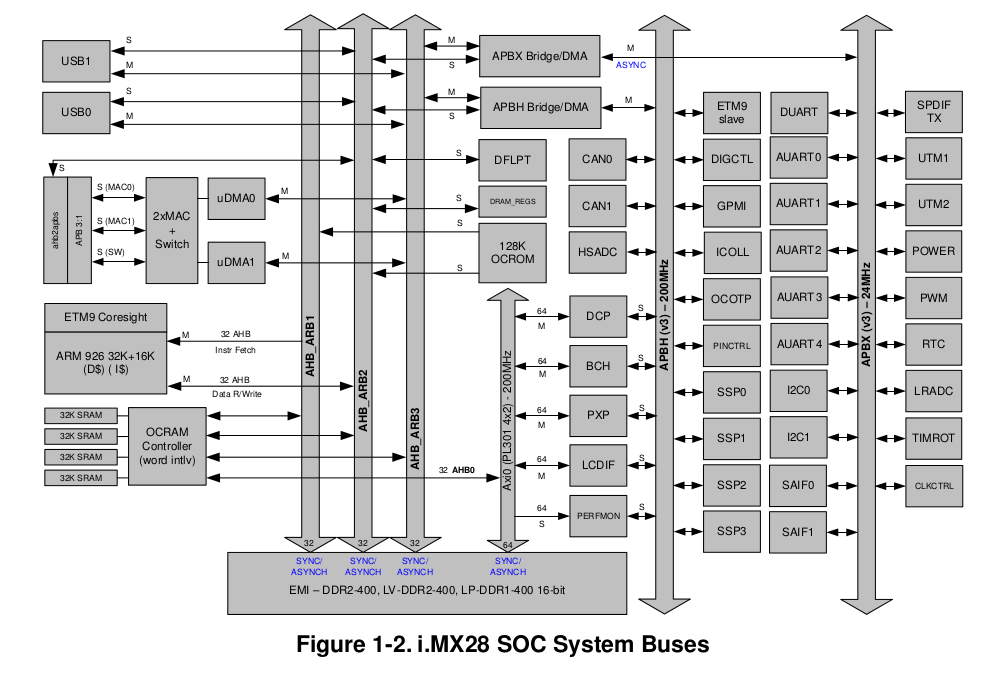
\includegraphics[width=\textwidth]{imx28-busses.png}
  \end{center}
\end{frame}

\begin{frame}[fragile]{Device Tree organization: {\tt imx28-evk.dts}}
  \begin{block}{\code{arch/arm/boot/dts/imx28-evk.dts}}
  \begin{minted}[fontsize=\scriptsize]{perl}
/ {
        model = "Freescale i.MX28 Evaluation Kit";
        compatible = "fsl,imx28-evk", "fsl,imx28";

        memory {
                reg = <0x40000000 0x08000000>;
        };


        apb@80000000 {
                apbh@80000000 { ... };
                apbx@80040000 { ... };
        };

        ahb@80080000 { ... };

        sound { ... };
        leds { ... };
        backlight { ... };
};
\end{minted}
\end{block}
\end{frame}

\begin{frame}[fragile]{Top-level {\tt compatible} property}
  \begin{itemize}
  \item The top-level \code{compatible} property typically defines a
    compatible string for the board, and then for the SoC.
  \item Values always given with the most-specific first, to
    least-specific last.
  \item Used to match with the \code{dt_compat} field of the
    \code{DT_MACHINE} structure:
    \begin{block}{}
      \begin{minted}[fontsize=\tiny]{c}
static const char *mxs_dt_compat[] __initdata = {
        "fsl,imx28",
        "fsl,imx23",
        NULL,
};

DT_MACHINE_START(MXS, "Freescale MXS (Device Tree)")
        .dt_compat      = mxs_dt_compat,
        [...]
MACHINE_END
      \end{minted}
    \end{block}
  \item Can also be used within code to test the machine:
    \begin{block}{}
      \begin{minted}[fontsize=\tiny]{c}
if (of_machine_is_compatible("fsl,imx28-evk"))
        imx28_evk_init();
      \end{minted}
    \end{block}
  \end{itemize}
\end{frame}

\begin{frame}{Bus, address cells and size cells}
  Inside a bus, one typically needs to define the following
  properties:
  \begin{itemize}
  \item A \code{compatible} property, which identifies the bus
    controller (in case of I2C, SPI, PCI, etc.). A special value
    \code{compatible = "simple-bus"} means a simple memory-mapped bus
    with no specific handling or driver. Child nodes will be
    registered as {\em platform devices}.
  \item The {\usebeamercolor[fg]{code} {\tt \#address-cells}} property
    indicate how many cells (i.e 32 bits values) are needed to form
    the base address part in the \code{reg} property.
  \item The {\usebeamercolor[fg]{code} {\tt \#size-cells}} is the
    same, for the size part of the \code{reg} property.
  \item The \code{ranges} property can describe an {\em address
      translation} between the child bus and the parent bus. When
    simply defined as \code{ranges;}, it means that the translation is
    an identity translation.
  \end{itemize}
\end{frame}

\begin{frame}[fragile]{\code{simple-bus}, address cells and size cells}
  \begin{block}{}
\begin{minted}[fontsize=\scriptsize]{perl}
apbh@80000000 {
        compatible = "simple-bus";
        #address-cells = <1>;
        #size-cells = <1>;
        reg = <0x80000000 0x3c900>;
        ranges;

        [...]

        hsadc: hsadc@80002000 {
                reg = <0x80002000 0x2000>;
                interrupts = <13>;
                dmas = <&dma_apbh 12>;
                dma-names = "rx";
                status = "disabled";
        };

        [...]
};
\end{minted}
\end{block}
\end{frame}

\begin{frame}[fragile]{I2C bus, address cells and size cells}
  \begin{block}{}
\begin{minted}[fontsize=\scriptsize]{perl}
i2c0: i2c@80058000 {
        #address-cells = <1>;
        #size-cells = <0>;
        compatible = "fsl,imx28-i2c";
        reg = <0x80058000 0x2000>;
        interrupts = <111>;
        [...]

        sgtl5000: codec@0a {
                compatible = "fsl,sgtl5000";
                reg = <0x0a>;
                VDDA-supply = <&reg_3p3v>;
                VDDIO-supply = <&reg_3p3v>;
                clocks = <&saif0>;
        };

        at24@51 {
                compatible = "at24,24c32";
                pagesize = <32>;
                reg = <0x51>;
        };
};
\end{minted}
\end{block}
\end{frame}

\begin{frame}{Interrupt handling}
  \begin{itemize}
  \item \code{interrupt-controller;} is a boolean property that
    indicates that the current node is an interrupt controller.
  \item {\usebeamercolor[fg]{code} {\tt \#interrupt-cells}} indicates
    the number of cells in the \code{interrupts} property for the
    interrupts managed by the selected interrupt controller.
  \item \code{interrupt-parent} is a {\em phandle} that points to the
    interrupt controller for the current node. There is generally a
    top-level \code{interrupt-parent} definition for the main
    interrupt controller.
  \end{itemize}
\end{frame}

\begin{frame}[fragile]{Interrupt example: {\tt imx28.dtsi}}
  \begin{block}{}
    \begin{minted}[fontsize=\scriptsize]{perl}
/ {
    interrupt-parent = <&icoll>;
    apb@80000000 {
        apbh@80000000 {
            icoll: interrupt-controller@80000000 {
                compatible = "fsl,imx28-icoll", "fsl,icoll";
                interrupt-controller;
                #interrupt-cells = <1>;
                reg = <0x80000000 0x2000>;
            };

            ssp0: ssp@80010000 {
                [...]
                interrupts = <96>;
            };
        };
    };
};
    \end{minted}
  \end{block}
\end{frame}

\begin{frame}{A more complicated example on Tegra 20}
  \begin{center}
    \includegraphics[width=\textwidth]{tegra20-dt-example.pdf}
  \end{center}
\end{frame}

\begin{frame}[fragile]{Interrupt example: {\tt tegra20.dtsi}}
  \begin{block}{}
    \begin{minted}[fontsize=\tiny]{perl}
/ {
  interrupt-parent = <&intc>;

  intc: interrupt-controller {
    compatible = "arm,cortex-a9-gic";
    reg = <0x50041000 0x1000 0x50040100 0x0100>;
    interrupt-controller;
    #interrupt-cells = <3>;
  };

  i2c@7000c000 {
    compatible = "nvidia,tegra20-i2c";
    reg = <0x7000c000 0x100>;
    interrupts = <GIC_SPI 38 IRQ_TYPE_LEVEL_HIGH>;
    #address-cells = <1>;
    #size-cells = <0>;
    [...]
  };

  gpio: gpio {
      compatible = "nvidia,tegra20-gpio";
      reg = <0x6000d000 0x1000>;
      interrupts = <GIC_SPI 32 IRQ_TYPE_LEVEL_HIGH>, <GIC_SPI 33 IRQ_TYPE_LEVEL_HIGH>,
           [...], <GIC_SPI 89 IRQ_TYPE_LEVEL_HIGH>;
      #gpio-cells = <2>;
      gpio-controller;
      #interrupt-cells = <2>;
      interrupt-controller;
  };
};
\end{minted}
\end{block}
\end{frame}

\begin{frame}[fragile]{Interrupt example: {\tt tegra20-harmony.dts}}
\begin{block}{}
  \begin{minted}[fontsize=\scriptsize]{perl}
i2c@7000c000 {
  status = "okay";
  clock-frequency = <400000>;

  wm8903: wm8903@1a {
    compatible = "wlf,wm8903";
    reg = <0x1a>;
    interrupt-parent = <&gpio>;
    interrupts = <TEGRA_GPIO(X, 3) IRQ_TYPE_LEVEL_HIGH>;

    gpio-controller;
    #gpio-cells = <2>;

    micdet-cfg = <0>;
    micdet-delay = <100>;
    gpio-cfg = <0xffffffff 0xffffffff 0 0xffffffff 0xffffffff>;
  };
};
\end{minted}
\end{block}
\end{frame}

\begin{frame}{DT is hardware description, not configuration}
  \begin{itemize}
  \item The Device Tree is really a hardware description language.
  \item It should {\bf describe the hardware layout}, and how it works.
  \item But it should {\bf not describe which particular hardware
      configuration} you're interested in.
  \item As an example:
    \begin{itemize}
    \item You may describe in the DT whether a particular piece of hardware
      supports DMA or not.
    \item But you may not describe in the DT if you {\em want} to use
      DMA or not.
    \end{itemize}
  \end{itemize}
\end{frame}

\begin{frame}{DT bindings as an ABI}
  \begin{itemize}
  \item Since the DT is OS independent, it should also be stable.
  \item The original idea is that DTBs can be flashed on some devices
    by the manufacturer, so that the user can install whichever
    operating system (s)he wants.
  \item Once a Device Tree binding is defined, and used in DTBs, it
    should no longer be changed anymore. It can only be extended.
  \item This normally means that {\bf Device Tree bindings become part
      of the kernel ABI}, and it should be handled with the same care.
  \item However, kernel developers are realizing that this is really
    hard to achieve and slowing down the integration of drivers.
    \begin{itemize}
    \item The ARM Kernel Mini-summit discussions have relaxed those
      rules.
    \item There will be additional discussions during the Kernel
      Summit, with final conclusions published afterwards.
    \end{itemize}
  \end{itemize}
\end{frame}

\begin{frame}{Basic guidelines for binding design}
  \begin{itemize}
  \item {\bf A precise compatible string is better than a vague one}
    \begin{itemize}
    \item You have a driver that covers both variants T320 and T330 of
      your hardware. You may be tempted to use \code{foo,t3xx} as your
      compatible string.
    \item Bad idea: what if T340 is slightly different, in an
      incompatible way? You'd better use \code{foo,t320} for both T320
      and T330.
    \end{itemize}
  \item {\bf Do not encode too much hardware details in the DT}
    \begin{itemize}
    \item When two hardware variants are quite similar, some
      developers are tempted to encode all the differences in the DT,
      including register offsets, bit masks or offsets.
    \item Bad idea: it makes the binding more complex, and therefore
      less resilient to future changes. Instead, use two different
      compatible strings and handle the differences in the driver.
    \end{itemize}
  \end{itemize}
\end{frame}

\begin{frame}{Future directions}
  \begin{itemize}
  \item Dynamic {\em Device Tree}, with the principle of {\em
      overlay}. Partially merged in 3.19.
  \item A {\bf tool to validate DTS against bindings}
    \begin{itemize}
    \item Currently, the DT compiler only makes syntax checks, no
      conformance checks against bindings.
    \item Proposal from Benoit Cousson and Fabien Parent, also from
      Tomasz Figa.
    \item No progress since several months.
    \end{itemize}
  \item {\bf Take out the Device Tree source files from the kernel tree}
    \begin{itemize}
    \item DTs are OS independent, so they can be used for other
      purposes than just Linux. They are already used by Barebox or
      U-Boot.
    \item Having them outside of the kernel reduces the amount of {\em
        churn} in the kernel source.
    \item But is IMO likely to cause a huge number of compatibility
      issues.
    \end{itemize}
  \end{itemize}
\end{frame}

\begin{frame}{References}
  \begin{itemize}
  \item Power.orgTM Standard for Embedded Power Architecture
    Platform Requirements (ePAPR),
    \url{http://www.power.org/resources/downloads/Power_ePAPR_APPROVED_v1.0.pdf}
  \item DeviceTree.org website, \url{http://www.devicetree.org}
  \item Device Tree documentation in the kernel sources,
    \code{Documentation/devicetree}
  \item The Device Tree kernel mailing list,
    \code{http://dir.gmane.org/gmane.linux.drivers.devicetree}
  \end{itemize}
\end{frame}

\begin{frame}
  \begin{center}
  \Huge
  Questions?\\
  \vspace{1.5cm}
  \huge
  Thomas Petazzoni\\
  \large
  \vspace{0.5cm}
  \code{thomas.petazzoni@bootlin.com}
  \vspace{0.5cm}
  \newline Slides under CC-BY-SA 3.0\\
  \scriptsize
  \url{http://bootlin.com/pub/conferences/2014/elc/petazzoni-device-tree-dummies/}
  \end{center}
\end{frame}

\begin{frame}
  \begin{center}
    \Huge
    Backup slides
  \end{center}
\end{frame}

\begin{frame}{Clock tree example, Marvell Armada XP}
  \begin{center}
    \includegraphics[width=\textwidth]{armada-clock-tree.pdf}
  \end{center}
\end{frame}

\begin{frame}[fragile]{Clock examples: instantiating clocks}
  \begin{block}{}
    \begin{minted}[fontsize=\tiny]{perl}
soc {
    coreclk: mvebu-sar@18230 {
        compatible = "marvell,armada-xp-core-clock";
        reg = <0x18230 0x08>;
        #clock-cells = <1>;
    };

    cpuclk: clock-complex@18700 {
        #clock-cells = <1>;
        compatible = "marvell,armada-xp-cpu-clock";
        reg = <0x18700 0xA0>;
        clocks = <&coreclk 1>;
    };

    gateclk: clock-gating-control@18220 {
        compatible = "marvell,armada-xp-gating-clock";
        reg = <0x18220 0x4>;
        clocks = <&coreclk 0>;
        #clock-cells = <1>;
    };
}

clocks {
    /* 25 MHz reference crystal */
    refclk: oscillator {
          compatible = "fixed-clock";
          #clock-cells = <0>;
          clock-frequency = <25000000>;
    };
};
  \end{minted}
\end{block}
\end{frame}

\begin{frame}[fragile]{Clock examples: consuming clocks}
  \begin{block}{CPU, using a \code{cpuclk}}
    \begin{minted}[fontsize=\tiny]{perl}
cpu@0 {
        device_type = "cpu";
        compatible = "marvell,sheeva-v7";
        reg = <0>;
        clocks = <&cpuclk 0>;
};
\end{minted}
  \end{block}

  \begin{block}{Timer, using either a \code{coreclk} or \code{refclk}}
    \begin{minted}[fontsize=\tiny]{perl}
timer@20300 {
        compatible = "marvell,armada-xp-timer";
        clocks = <&coreclk 2>, <&refclk>;
        clock-names = "nbclk", "fixed";
};
\end{minted}
  \end{block}

  \begin{block}{USB, using a \code{gateclk}}
    \begin{minted}[fontsize=\tiny]{perl}
usb@52000 {
        compatible = "marvell,orion-ehci";
        reg = <0x52000 0x500>;
        interrupts = <47>;
        clocks = <&gateclk 20>;
        status = "disabled";
};
\end{minted}
  \end{block}

\end{frame}

\begin{frame}[fragile]{{\em pinctrl} binding: consumer side}
  \begin{itemize}
  \item The {\em pinctrl} subsystem allows to manage pin muxing.
  \item In the Device Tree, devices that need pins to be muxed in a
    certain way must declare the {\em pinctrl} configuration they
    need.
  \item The \code{pinctrl-<n>} properties allow to give the list of
    {\em pinctrl} configuration needed for a certain {\em state} of
    the device.
  \item The \code{pinctrl-names} property allows to give a name to
    each state.
  \item When a device is probed, its \code{default} {\em pinctrl}
    state is requested automatically.
    \begin{block}{}
      \begin{minted}[fontsize=\tiny]{perl}
ssp0: ssp@80010000 {
    pinctrl-names = "default";
    pinctrl-0 = <&mmc0_8bit_pins_a
                 &mmc0_cd_cfg &mmc0_sck_cfg>;
    [...]
};
\end{minted}
    \end{block}
  \end{itemize}
\end{frame}

\begin{frame}[fragile]{{\em pinctrl} configurations}
  \begin{itemize}
  \item A {\em pinctrl} configuration provides a list of pins and
    their configuration.
  \item Such configurations are defined as {\em sub-nodes} of the {\em
      pinctrl device}, either at the SoC-level, or board-level.
  \item The binding for such configurations is highly dependent on the
    specific {\em pinctrl} driver being used.
  \end{itemize}
  \begin{columns}
    \column{0.5\textwidth}
    \begin{block}{i.MX28}
      \begin{minted}[fontsize=\tiny]{perl}
mmc0_8bit_pins_a: mmc0-8bit@0 {
   fsl,pinmux-ids = <
      0x2000 /* MX28_PAD_SSP0_DATA0__SSP0_D0 */
      0x2010 /* MX28_PAD_SSP0_DATA1__SSP0_D1 */
      [...]
      0x2090 /* MX28_PAD_SSP0_DETECT__SSP0_... */
      0x20a0 /* MX28_PAD_SSP0_SCK__SSP0_SCK */
   >;
   fsl,drive-strength = <1>;
   fsl,voltage = <1>;
   fsl,pull-up = <1>;
};
\end{minted}
\end{block}
\column{0.5\textwidth}
    \begin{block}{Marvell Kirkwood}
      \begin{minted}[fontsize=\tiny]{perl}
pmx_nand: pmx-nand {
   marvell,pins = "mpp0", "mpp1", "mpp2", "mpp3",
                  "mpp4", "mpp5", "mpp18",
                  "mpp19";
   marvell,function = "nand";
};
        \end{minted}
      \end{block}
  \end{columns}
\end{frame}

\end{document}
